% basic nastaveni
\documentclass[12pt]{article}
\setlength{\parindent}{0pt}
\setlength{\parskip}{1em}
\usepackage[utf8]{inputenc}
\usepackage[czech]{babel}
\usepackage[T1]{fontenc}
\usepackage{graphics}
\usepackage{caption}
\usepackage{hyperref}
\usepackage{dsfont}
\usepackage{color}
\usepackage{float}
\usepackage{enumitem}
\usepackage{graphicx}

% matematicke package
\usepackage{tikz-cd}
\usetikzlibrary{babel}
\usepackage{amsmath}
\usepackage{amssymb}
\usepackage{amsfonts}
\usepackage{amssymb}
\usepackage{geometry}
\geometry{margin=2.5cm}
\usepackage{pgfplots}
\pgfplotsset{compat=1.18}
\title{Maturitní otázka číslo 2: Množiny}
\author{}
\date{}

\begin{document}
\maketitle
\subsection*{Základní pojmy}
\begin{itemize}[itemsep = 2pt]
    \item \textbf{Množina} je soubor rozlišitelných prvků, která je jednoznačně určena svými prvky a nezáleží na pořadí prvků
    \item \textbf{Prvek množiny} značíme jako $x \in A$, což znamená, že prvek $x$ patří do množiny $A$. Pokud prvek nepatří do množiny, značíme to jako $x \notin A$.
    \item \textbf{Mohutnost(velikost) množiny} se značí jako $|A|$ a udává počet prvků v množině $A$.
    \item \textbf{Prázdná množina} se značí jako $\emptyset$ a neobsahuje žádné prvky.

\end{itemize}
\subsection*{Vztahy mezi množinami}
\begin{itemize}[itemsep = 2pt]
    \item \textbf{Podmnožina} she značí jako $A \subseteq B$, pokud každý prvek z A patří zároveň do B. \textbf{Vlastní podmnožina} se značí A $\subset$ B, znamená to, že A je podmnožinou B, ale $A \neq B$, tedy v B je alespoň jeden prvek navíc. (přijde mi, že tohle kritérium Pazi úplně nenásleduje, ale nevim)
    \item \textbf{Rovnost množin} se značí jako $A = B$ a jsou si rovny, pokud obsahují stejné prvky, formálně $A \subseteq B$ a $B \subseteq A$
    \item \textbf{Průnik} množin $A$ a $B$ se značí jako $A \cap B$ a obsahuje všechny prvky, které jsou společné pro obě množiny. Formálně $A \cap B = \{x | x \in A \land x \in B\}$
    \item \textbf{Disjunktní množiny} jsou množiny, které nemají žádný společný prvek. Jejich průnikem je prázdná množina $A\cap B = \emptyset$
    \item \textbf{Sjednocení} množin $A$ a $B$ se značí jako $A \cup B$ a obsahuje všechny prvky, které jsou v A nebo v B. Prvky, které se nacházejí v obou množinách jsou zahrnuty pouze jednou.
    \item \textbf{Rozdíl} množin se značí jako $A \setminus B$ nebo $A - B$ a obsahuje všechny prvky, které jsou v A, ale nejsou v B. \textbf{Není komutativní}
    \item \textbf{Doplněk množiny} A se značí jako $A'$ nebo $A'_b$ a obsahuje všechny prvky, které nejsou v A, ale jsou v množině B v našem případě.
\end{itemize}
\begin{figure}[H]
    \centering % Zarovná obrázek na střed
    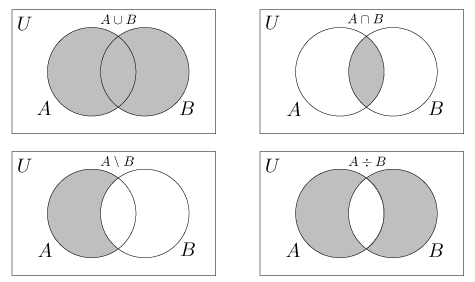
\includegraphics[width=0.8\textwidth]{pictures/mnoziny.png} % Nahraďte 'obrazek.png' názvem vašeho obrázku
    \caption*{Vennův diagram znázorňující výše vysvětlené operace s množinami}
    \label{fig:muj_obrazek} % Slouží pro křížové odkazy v textu
\end{figure}

\subsection*{Kartézský součin}
Značí se jako $A \times B$ a obsahuje všechny uspořádané dvojice $(a, b)$, kde $a \in A$ a $b \in B$. Pokud bychom tedy měli množinu $A = \{1,2,3\}$ a množinu $B = \{x,y\}$, jejich kartézský součin bude následovný: $A \times B = \{(1,x), (1,y), (2,x), (2,y), (3,x), (3,y)\}$. Kartézský součin není komutativní, tedy $A \times B \neq B \times A$.

Počet prvků v kartézském součinu je roven součinu počtů prvků jednotlivých množin, tedy $|A| \times |B|$

\textbf{Kartézská mocnina} je speciální případ kartézského součinu, kdy se množina $A$ násobí sama sebou $n$-krát, značí se jako \textbf{$A^n$} a obsahuje všechny uspořádané n-tice $(a_1, a_2, ..., a_n)$, kde každý prvek $a_i$ pochází z množiny $A$. Počet prvků v kartézské mocnině je roven $|A|^n$.

Jeden z příkladů použití kartézského součinu je jeho využití pro definici kartézské roviny $\mathbb{R}^2 = \mathbb{R} \times \mathbb{R}$, kde $\mathbb{R}$ je množina reálných čísel. Každý bod v této rovině je reprezentován uspořádanou dvojicí $(x, y)$, kde $x$ a $y$ jsou reálná čísla.

Příklad: Znázorněte kartézský součin množin $\mathbb{N} \times \mathbb{R}$, kde $\mathbb{N}$ je množina přirozených čísel. 

Řešení: Tento kartézský součin by byl reprezentován jako nekonečně mnoho svislých čar na kartézské rovině, kde každá čára odpovídá jednomu přirozenému číslu. Na ose x by byly znázorněny přirozená čísla, zatímco na ose y by byly reálná čísla. 

\begin{figure}[H]
    \centering
    \begin{tikzpicture}
        \begin{axis}[
            axis lines = middle,
            xlabel = {$x$}, 
            ylabel = {$y$},
            xmin = -1, xmax = 7, % Osa x končí kousek za 6, aby bylo místo na tečky
            ymin = -3, ymax = 3,   % Rozsah osy y
            xtick = {1, 2, 3, 4, 5, 6}, % Vykreslíme čísla na ose x
            ytick = {-2, -1, 1, 2},     % Vykreslíme čísla na ose y
            grid = none % Zde mřížku vypneme, aby nerušila samotné řešení
        ]
        
        % Vykreslení svislých čar pomocí cyklu
        % \i postupně nabývá hodnot 1, 2, 3, 4, 5, 6
        \pgfplotsinvokeforeach{1,2,3,4,5,6}{
            \draw[blue, thick] (#1, -3) -- (#1, 3);
        }
        
        % Přidání tří teček, které naznačují, že množina N pokračuje do nekonečna
        \node[right] at (6.3, -0.5) {\dots};
        \node [below left] at (0,0) {$0$};
        
        \end{axis}
    \end{tikzpicture}
    \caption*{Graf znázorňující řešení: Kartézský součin $\mathbb{N} \times \mathbb{R}$}
\end{figure}


\subsection*{Relace}
Relace R nad množinami A a B je libovolná podmnožina kartézského součinu $A \times B $. Relace může být i inverzní, značí se jako $R^{-1}$ a všechny dvojice jsou $(b, a)$.

\subsubsection*{Vlastnosti relací}
\begin{itemize}[itemsep = 2pt]
    \item \textbf{Symetrická} je pokud je první prvek v relaci s druhým a druhý s prvním. Tedy pokud $(a, b) \in R$, pak také $(b, a) \in R$.
    \item \textbf{Tranzitivní} je pokud je první prvek v relaci s druhým a a druhý v relaci s třetím, pak první je v relaci s třetím. Tedy pokud $(a,b) \in R$ a $(b,c) \in R$ pak také $(a,c) \in R$. 
    \item \textbf{Reflexivní} je pokud je každý prvek v relaci sám se sebou. Tedy pro každé $a \in A$, $(a, a) \in R$.
\end{itemize}
Například kartézská mocnina reálných čísel $\mathbb{R}^2$ je reflexivní, symetrická a tranzitivní relace. 
\begin{itemize}[itemsep = 2pt]
    \item \textbf{Relace ekvivalence} je relace, která je reflexivní, symetrická a tranzitivní. Tato relace se objevuje například u rovnoběžnosti(když $a \parallel b$ a $b \parallel c$ pak $a \parallel c$) nebo u rovnosti (když $a = b$ a $b = c$ pak $a = c$).)
    \item \textbf{Relace uspořádání} je relace, která je antisymetrická a tranzitivní. Objevuje se například u porovnávání čísel (když $a \leq b$ a $b \leq c$ pak $a \leq c$)
\end{itemize}

\subsection*{Zobrazení}
Definice: Zobrazení $f$ z množiny $A$ do množiny $B$ je předpis, který každému prvku $x \in A$ přiřazuje nejvýše jeden prvek $y \in B$. Zobrazení je tudíž zprava jednoznačné. 

Zobrazení se zapisuje následovně: $f: A \rightarrow B$ a říkáme, že $f$ zobrazuje množinu $A$ do množiny $B$. Prvek $y$ se nazývá obrazem prvku $x$ a značí se jako $f(x) = y$. Prvek $x$ se nazývá vzorem prvku $y$.
\begin{itemize}[itemsep = 2pt]
    \item \textbf{Obor hodnot} je množina všech obrazů pro které existuje vzor v možině  $A$, značí $H_f$. Pozor, není vždy totožný s množinou $B$.
    \item \textbf{Definiční obor} je množina všechn vzorů, pro které existuje obraz v množině $B$, značí se $D_f$.
\end{itemize}
Existují různé typy zobrazení, které se liší podle toho jak jsou k sobě přiřazeny vzory a obrazy
\begin{itemize}[itemsep = 2pt]
    \item \textbf{Injekce} je zobrazení, které se také nazývá prosté zobrazení. Je charakteristické tím, že každé dva různé prvky z množiny $A$ jsou zobrazeny na různé prvky v množině $B$. Jako diagram pomocí šipek by vypadalo následovně: \\
    
    \begin{tikzcd}[row sep = tiny]
        1 \arrow[rd] & 1 \\
        2 \arrow[rd] & 2 \\
        3 \arrow[ruu] & 3 \\
        & 4\\
    \end{tikzcd}
    \item \textbf{Surjekce} je zobrazení, které se může nazývat zobrazení „na". Obor hodnot se je stejný jako množina $B$, tedy každý prvek z $B$ má alespoň jeden vzor v $A$. Přílad tohoto zobrazení by vypadal následovně:\\
    \begin{tikzcd}[row sep = tiny]
        1 \arrow[rd] & 1 \\
        2 \arrow[rd] & 2 \\
        3 \arrow[ruu] & 3 \\
        4 \arrow[ru]\\
    \end{tikzcd}
    \item \textbf{Bijekce} je zobrazení, které je vzájemně jednoznačné, tedy každému prvku z $A$ je přiřazen právě jeden prvek z $B$ a zároveň každý prvek z $B$ má právě jeden vzor v $A$. Toto zobrazení je zároveň injekcí i surjekcí a proto existuje jeho inverzí verze, která je zobrazením. Množina $A$ i $B$ musí mít stejnou mohutnost(počet prvků). Jeho příklad by vypadal následovně:\\
    \begin{tikzcd}[row sep = tiny]
        1 \arrow[r] & 1 \\
        2 \arrow[r] & 2 \\
        3 \arrow[rd] & 3 \\
        4 \arrow[ru] & 4\\
    \end{tikzcd}
\end{itemize}

\textbf{Složené zobrazení} se značí $g \circ f$. Pokud máme zobrazení $f: A \rightarrow B$ a $g: B \rightarrow C$, pak složené zobrazení $g \circ f$ je zobrazení z množiny $A$ do množiny $C$, které přiřazuje každému prvku $x \in A$ prvek $g(f(x)) \in C$.\\
\\
Příklad: Nechť $f: \mathbb{N} \rightarrow \mathbb{N}$ je zobrazení definované jako $f(x) = 2x$ a $g: \mathbb{N} \rightarrow \mathbb{N}$ je zobrazení definované jako $g(y) = y + 3$. Zapište zobrazení $f$ a $g$ a poté složené zobrazení $g \circ f$. U obou zobrazení určete jen první 4 prvky
\\
\\
Řešení: Prvních 5 prvků zobrazení $f$ je f = \{(1, 2), (2, 4), (3, 6), (4, 8)\} a první 4 prvky zobrazení $g$ je g = \{(1, 4), (2, 5), (3, 6), (4, 7)\}. Složené zobrazení $g \circ f$ je definováno jako $g(f(x)) = g(2x) = 2x + 3$. První 4 prvky složeného zobrazení $g \circ f$ je \{(1, 5), (2, 7), (3, 9), (4, 11)\}.
\\ složené zobrazení je také možné znázornit pomocí diagramu se šipkami.
\[
\begin{tikzcd}[row sep = tiny]
    1 \arrow[rd] &  1  & 1\\
    2 \arrow[ddr] &  2 \arrow[dddr] & 2\\
    3 \arrow[dddr] &  3  & 3\\
    4 \arrow[ddddr] &  4 \arrow[dddr] & 4\\
                & 5 & 5 \\
                & 6 \arrow[dddr] & 6 \\
                & 7 & 7 \\
                & 8 \arrow[dddr] & 8 \\
                & & 9\\
                & & 10\\
                & & 11\\
\end{tikzcd}
\]
Pomocí šipek prostě zapíši sloupce s čísly, první dva pospojuji tak, jak mi vycházejí z předpisu 1. zobrazení, nebo výčtu prvků a pak pospojuji jen ty prvky ke kterým vede šipka s dalším sloupcem podle předpisu nebo výčtu prvků druhého zobrazení.
\newpage
A poslední příklad na závěr: Graficky znázorněte kartézský součin $A \times B$ množin \\$A = <-3, 1>$ a $B = <-2, 3>$ v množině $\mathbb{R}$. 

Řešení: 
\begin{figure}[H]
    \centering
    \begin{tikzpicture}
        \begin{axis}[
            axis lines = middle, % Nastaví osy tak, aby se křížily uprostřed (jako kříž)
            xlabel = {$x$},      % Popisek osy x
            ylabel = {$y$},      % Popisek osy y
            xmin = -4, xmax = 2, % Rozsah osy x
            ymin = -3, ymax = 4, % Rozsah osy y
            xtick = {-4, -3, -2, -1, 0, 1, 2}, % Čísla, která se na ose x zobrazí
            ytick = {-3, -2, -1, 0, 1, 2, 3, 4}, % Čísla, která se na ose y zobrazí
            grid = both,         % Zapne pomocnou mřížku
            grid style = {dashed, gray!30} % Mřížka bude čárkovaná a světle šedá
        ]
        
        % Tady vykreslíme ten čtverec!
        % 'fill=blue!20' znamená modrá barva s průhledností 20 %
        % 'draw=blue' udělá tmavě modrý okraj
        \filldraw[fill=blue, fill opacity=0.3,draw=blue, thick] (-3, -2) rectangle (1,3);
        \node [below left] at (0,0) {$0$};
        \end{axis}
    \end{tikzpicture}
    \caption*{Znázornění kartézského součinu jako plochy}
\end{figure}




\end{document}